\documentclass[12pt]{article}
\usepackage[spanish]{babel}
\usepackage{listings}
\usepackage{array}
\usepackage{graphicx}

%opening
\title{{\Huge \textbf{Mips}}}
\author{Samuel Primera CI: 31.129.684}

\begin{document}
	\maketitle
	
	
	\section{Operandos Mips}
	
	\subsection{32 Registros}
	
	Localizaciones rápidas para los datos. En MIPS, los datos deben estar en los registros para realizar operaciones aritméticas. El registro MIPS \$zero es siempre igual a O. El registro \$ at está reservado por el ensamblador para manejar constantes grandes. Ejemplo:
	
	\begin{center}
		\$s0-\$s7. \$t0-\$t9.\\
		\$zero. \$a0-\$a3.\\
		\$vO-\$v1. \$gp. \$fp. \$sp.\\
		\$ra. \$at\\
	\end{center}
	
	\subsection{$2^{30}$ Palabras de memoria}
	
	Accesibles solamente por instrucciones de transferencia de datos. MIPS utiliza direcciones de byte, de modo que las direcciones de palabras consecutivas se diferencian en 4. La memoria guarda las estructuras de datos, las tablas y los registros desbordados (guardados). Ejemplo:
	
	\begin{center}
		Memory[0],\\
		Memory[4], ... ,\\
		Memory[4294967292]
	\end{center}
	
	\section{Lenguaje Ensamblador Mips}
	
	\begin{flushleft}
		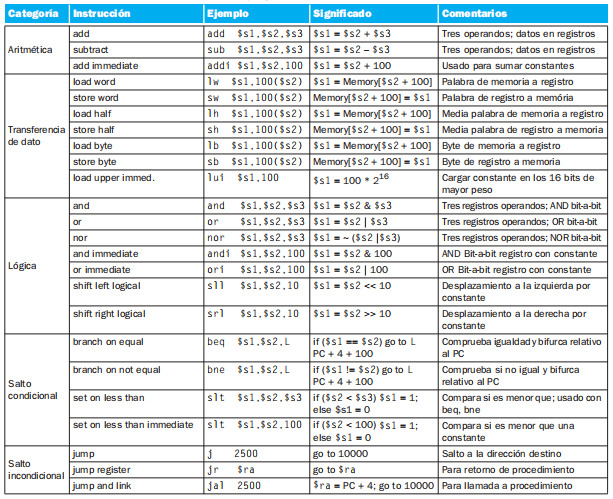
\includegraphics[width=1.2\linewidth]{LenguajeEsambladorMips.jpg}
		\end{flushleft}
	
\end{document}